% !TeX program = xelatex
% Compile twice with XeLaTeX to update the table of contents and references.
\documentclass[11pt,letterpaper]{article}
\usepackage[letterpaper,top=0.78in,bottom=0.72in,left=0.82in,right=0.82in,headheight=15pt]{geometry}
\usepackage{fontspec}
% Use fontspec's bundled Latin Modern defaults so the source remains portable
% across standard TeX Live installations.
\usepackage{microtype}
\usepackage{booktabs,longtable,tabularx,array,multirow}
\usepackage[table]{xcolor}
\usepackage{enumitem}
\usepackage{fancyhdr}
\usepackage{titlesec}
\usepackage{needspace}
\usepackage{tikz}
\usetikzlibrary{arrows.meta,positioning,calc,fit}
\usepackage{graphicx}
\usepackage{caption}
\usepackage{hyperref}
\usepackage{bookmark}
\usepackage{url}

\definecolor{Ink}{HTML}{111827}
\definecolor{Muted}{HTML}{5B6470}
\definecolor{AcademicBlue}{HTML}{8C1515}
\definecolor{MidBlue}{HTML}{B1040E}
\definecolor{SoftBlue}{HTML}{F8ECEC}
\definecolor{SoftGray}{HTML}{F4F5F7}
\definecolor{Grid}{HTML}{D9D9D9}
\definecolor{ExactGreen}{HTML}{3E7A65}
\definecolor{TheoremBrown}{HTML}{8C6A3B}
\definecolor{NumericalRed}{HTML}{9A5B61}
\definecolor{MixedPurple}{HTML}{6D6278}

\hypersetup{
  colorlinks=true,
  linkcolor=AcademicBlue,
  urlcolor=AcademicBlue,
  citecolor=AcademicBlue,
  pdftitle={How Much Can LLMs Help Solve Mixed-Integer Programs?},
  pdfsubject={Evidence from 112 open MIPLIB instances},
  pdfkeywords={LLM, MIPLIB, MILP, exact algorithms, proof certificates, optimization}
}
\urlstyle{same}
\setlength{\parindent}{0pt}
\setlength{\parskip}{5.5pt plus 1pt minus 0.5pt}
\setlength{\emergencystretch}{2em}
\widowpenalty=10000
\clubpenalty=10000
\displaywidowpenalty=10000
\raggedbottom

\titleformat{\section}{\needspace{5\baselineskip}\sffamily\bfseries\Large\color{black}}{\thesection}{0.65em}{}
\titleformat{\subsection}{\needspace{4\baselineskip}\sffamily\bfseries\large\color{black}}{\thesubsection}{0.6em}{}
\titleformat{\subsubsection}{\needspace{3\baselineskip}\sffamily\bfseries\normalsize\color{black}}{\thesubsubsection}{0.5em}{}
\titlespacing*{\section}{0pt}{16pt plus 2pt}{6pt}
\titlespacing*{\subsection}{0pt}{11pt plus 1pt}{4pt}
\titlespacing*{\subsubsection}{0pt}{8pt}{3pt}

\setlist[itemize]{leftmargin=1.45em,itemsep=2pt,topsep=3pt}
\setlist[enumerate]{leftmargin=1.7em,itemsep=3pt,topsep=3pt}
\renewcommand{\arraystretch}{1.22}
\captionsetup{font={small,it},labelfont={bf},textfont={color=Muted},skip=5pt}

\pagestyle{fancy}
\fancyhf{}
\fancyhead[L]{\sffamily\footnotesize\color{Muted}LLM4MIP Capability Study}
\fancyhead[R]{\sffamily\footnotesize\color{Muted}Evidence through 18 September 2026 UTC}
\fancyfoot[C]{\sffamily\footnotesize\color{Muted}\thepage}
\renewcommand{\headrulewidth}{0pt}
\renewcommand{\footrulewidth}{0pt}

\newcommand{\code}[1]{\texttt{\detokenize{#1}}}
\newcommand{\tighttable}{\small\setlength{\tabcolsep}{5pt}\renewcommand{\arraystretch}{1.18}}
\newcommand{\sourcecite}[1]{\hyperref[#1]{[\ref*{#1}]}}

\newcommand{\WorkflowFigure}{%
\begin{figure}[htbp]
\centering
\resizebox{\textwidth}{!}{%
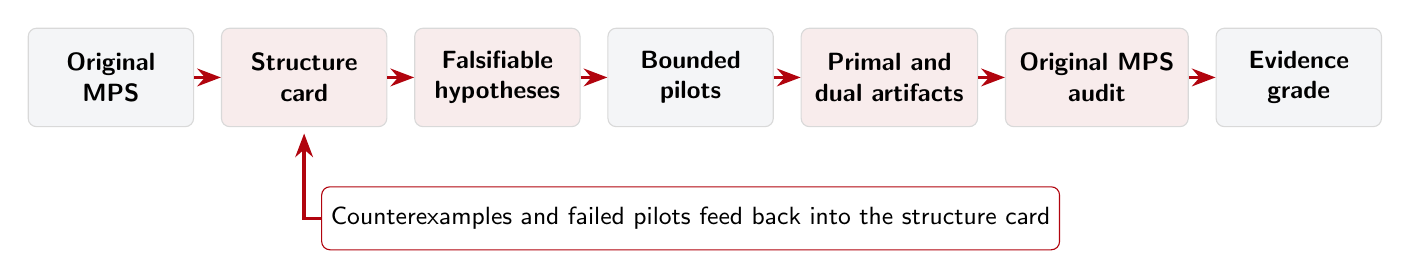
\begin{tikzpicture}[
  node distance=0.34cm,
  box/.style={draw=Grid,rounded corners=3pt,minimum width=2.1cm,minimum height=1.25cm,align=center,font=\sffamily\bfseries\small,inner sep=5pt},
  flow/.style={-{Stealth[length=3mm]},very thick,draw=MidBlue}
]
\node[box,fill=SoftGray] (mps) {Original\\MPS};
\node[box,fill=SoftBlue,right=of mps] (card) {Structure\\card};
\node[box,fill=SoftBlue,right=of card] (hyp) {Falsifiable\\hypotheses};
\node[box,fill=SoftGray,right=of hyp] (pilot) {Bounded\\pilots};
\node[box,fill=SoftBlue,right=of pilot] (art) {Primal and\\dual artifacts};
\node[box,fill=SoftBlue,right=of art] (audit) {Original MPS\\audit};
\node[box,fill=SoftGray,right=of audit] (grade) {Evidence\\grade};
\foreach \a/\b in {mps/card,card/hyp,hyp/pilot,pilot/art,art/audit,audit/grade}{\draw[flow] (\a) -- (\b);}
\node[draw=MidBlue,rounded corners=3pt,fill=white,font=\sffamily\small,align=center,below=0.75cm of pilot,minimum width=6.6cm,minimum height=0.8cm] (feedback) {Counterexamples and failed pilots feed back into the structure card};
\draw[flow] (feedback.west) -| ($(card.south)+(0,-0.08)$);
\end{tikzpicture}}
\caption{LLM-assisted research workflow with explicit falsification and return to the original MPS.}
\label{fig:workflow}
\end{figure}}

\newcommand{\CoverageFigure}{%
\begin{figure}[htbp]
\centering
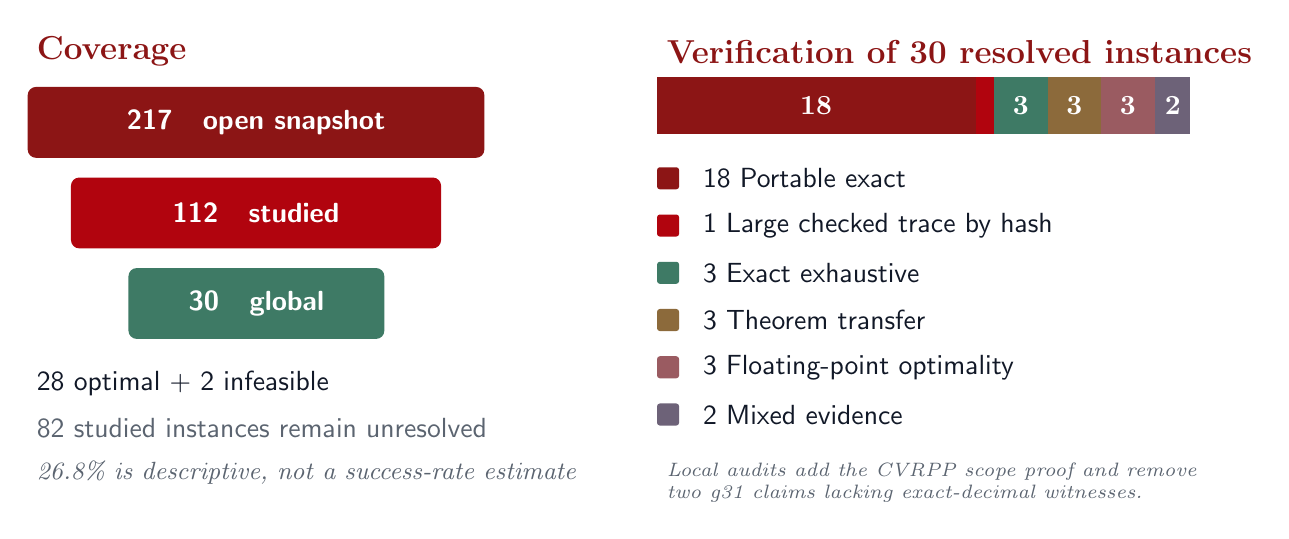
\begin{tikzpicture}[font=\sffamily]
  \node[anchor=west,font=\bfseries\large,text=AcademicBlue] at (0,5.7) {Coverage};
  \node[fill=AcademicBlue,text=white,rounded corners=3pt,minimum width=5.8cm,minimum height=0.9cm,anchor=west] at (0,4.8) {\bfseries 217\quad open snapshot};
  \node[fill=MidBlue,text=white,rounded corners=3pt,minimum width=4.7cm,minimum height=0.9cm,anchor=west] at (0.55,3.65) {\bfseries 112\quad studied};
  \node[fill=ExactGreen,text=white,rounded corners=3pt,minimum width=3.25cm,minimum height=0.9cm,anchor=west] at (1.28,2.5) {\bfseries 30\quad global};
  \node[anchor=west,text=Ink] at (0,1.48) {28 optimal + 2 infeasible};
  \node[anchor=west,text=Muted] at (0,0.92) {82 studied instances remain unresolved};
  \node[anchor=west,text=Muted,font=\itshape\small] at (0,0.35) {26.8\% is descriptive, not a success-rate estimate};

  \node[anchor=west,font=\bfseries\large,text=AcademicBlue] at (8.0,5.7) {Verification of 30 resolved instances};
  \fill[AcademicBlue] (8.0,4.65) rectangle +(4.05,0.72);
  \fill[MidBlue] (12.05,4.65) rectangle +(0.23,0.72);
  \fill[ExactGreen] (12.28,4.65) rectangle +(0.68,0.72);
  \fill[TheoremBrown] (12.96,4.65) rectangle +(0.68,0.72);
  \fill[NumericalRed] (13.64,4.65) rectangle +(0.68,0.72);
  \fill[MixedPurple] (14.32,4.65) rectangle +(0.45,0.72);
  \node[text=white,font=\bfseries] at (10.02,5.01) {18};
  \node[text=white,font=\bfseries] at (12.62,5.01) {3};
  \node[text=white,font=\bfseries] at (13.30,5.01) {3};
  \node[text=white,font=\bfseries] at (13.98,5.01) {3};
  \node[text=white,font=\bfseries] at (14.55,5.01) {2};
  \foreach \y/\c/\t in {3.95/AcademicBlue/{18  Portable exact},3.35/MidBlue/{1  Large checked trace by hash},2.75/ExactGreen/{3  Exact exhaustive},2.15/TheoremBrown/{3  Theorem transfer},1.55/NumericalRed/{3  Floating-point optimality},0.95/MixedPurple/{2  Mixed evidence}}{
    \fill[\c,rounded corners=1pt] (8.0,\y) rectangle +(0.28,0.28);
    \node[anchor=west,text=Ink] at (8.46,\y+0.14) {\t};
  }
  \node[anchor=west,text=Muted,font=\itshape\scriptsize,align=left] at (8.0,0.23) {Local audits add the CVRPP scope proof and remove\\two g31 claims lacking exact-decimal witnesses.};
\end{tikzpicture}
\caption{Frozen campaign coverage and evidence mix. Evidence classes preserve materially different dependencies.}
\label{fig:coverage}
\end{figure}}

\begin{document}
\hypersetup{pageanchor=false}
\begin{titlepage}
\thispagestyle{empty}
\vspace*{0.6in}
{\sffamily\bfseries\small\color{AcademicBlue} TECHNICAL REPORT\par}
\vspace{0.55in}
{\sffamily\bfseries\fontsize{28}{33}\selectfont\color{black} How Much Can LLMs Help Solve\\[3pt]Mixed-Integer Programs?\par}
\vspace{0.28in}
{\sffamily\fontsize{16}{20}\selectfont\color{Muted} Evidence from 112 open MIPLIB instances\par}
\vspace{0.65in}
{\fontsize{12.5}{18}\selectfont An evidence-graded study of where language models helped, where optimization backends still led, and which claims survived independent checking.\par}
\vfill
\begin{tabular}{@{}>{\sffamily\bfseries\color{Muted}}p{1.55in}p{4.8in}@{}}
Evidence date & 18 September 2026 UTC (17 September 2026 PDT)\\[5pt]
Published baseline & Commit \code{89a8abd} dated 16 September 2026\\[5pt]
Supplements & Local independent reviews dated 18 September 2026 UTC, not yet committed\\[5pt]
Audience & Mixed-integer optimization, exact algorithms, automated reasoning, and AI-assisted mathematics
\end{tabular}
\vspace{0.48in}

{\small\itshape\color{Muted} Prepared from the repository evidence archive. Official MIPLIB status was not live refreshed for this report.\par}
\end{titlepage}
\hypersetup{pageanchor=true}

\pagenumbering{roman}
\tableofcontents
\clearpage
\pagenumbering{arabic}
\section*{Executive summary}\addcontentsline{toc}{section}{Executive summary}

\textbf{Short answer.} Language models helped materially as research copilots, especially in semantic recovery, state-space redesign, experiment construction, falsification, and proof orchestration. They did not replace mixed-integer solvers, SAT engines, exact enumeration, or deterministic checking. The durable contribution of the \texttt{\detokenize{MIPLIB_openproblem}} project is the loop connecting LLM-generated hypotheses to independently checkable mathematical objects.

On the fixed 4 September 2026 snapshot of 217 officially open MIPLIB instances, the LLM-assisted campaign studied 112 current open instances and retained one historical calibration instance. The reconciled working tree supports 30 evidence-graded optimality or infeasibility results among the 112 studied instances: 28 optimal objective values and two infeasibility results. Eighty two studied instances remain globally unresolved. These numbers describe repository evidence, not updates to the official MIPLIB status pages, and they do not estimate a success probability because instance selection and research budgets were nonuniform \sourcecite{ref:repo}.

The repository also records 21 primal-bound improvements over existing MIPLIB v36 incumbent values, four first finite incumbents, and 41 dual-bound improvements relative to a frozen historical COPT 10 hour table. These are different, overlapping outcomes of the campaign. They are not 96 distinct wins, the primal and dual counts do not share a baseline, and the dual-bound comparison is not a same-hardware or same-budget solver benchmark.

The central findings are:

\begin{enumerate}
\item The LLM was most useful when it helped replace a large anonymous formulation by a smaller object: a tree, interval order, parity argument, finite cutoff, or proof-producing SAT instance.
\item Construction and proof remain different pipelines. A strong feasible solution does not prove a lower bound, and a lower bound does not supply a witness.
\item Solvers search and bound; deterministic checkers decide what survives. Reduced-model optimality, local infeasibility, and unchecked SAT unsatisfiability remain scoped statements.
\item The strongest direct comparison is mixed. In a nonrandomized 20-instance study, the structure arm produced stronger primal bounds under the archived $10^{-7}$ comparison rule and two exact global optimality certificates, while the comparison arm more often retained stronger numerical dual bounds.
\item The campaign counts establish research output, not sole LLM causation or a universal success rate.
\end{enumerate}

\section{Research question: what counts as help?}

The capability question has four outcome dimensions: a strict primal-bound improvement, a valid global dual-bound improvement, an evidence-supported optimality or infeasibility result, and proof portability. An LLM can contribute by interpreting the matrix, proposing a representation, designing a falsification test, or generating a checker. The claim itself counts only after the appropriate solver, exact computation, original-MPS audit, or proof replay succeeds.

For a minimization problem, the project uses the basic proof obligation \(\mathbf{LB \leq OPT \leq UB}\), with global optimality established only when a valid lower bound and a strictly feasible upper bound coincide.

The phrase \textbf{open instance} is frozen to the MIPLIB open list downloaded on 4 September 2026 \sourcecite{ref:miplib}. It means the official record at that snapshot did not report global optimality or infeasibility. It does not mean that no later local computation, external construction, or published theorem exists. The project therefore separates three statuses:

\begin{itemize}
\item the official status in the frozen MIPLIB snapshot;
\item the optimality or infeasibility result supported by the repository evidence; and
\item whether that result has a portable, independently replayable proof.
\end{itemize}

The numerical baseline for this report is the 16 September 2026 presentation \sourcecite{ref:deck} and the 14 September dual bound audit \sourcecite{ref:audit}, reconciled with the two 18 September working tree reviews. The 14 September audit upgrades the five \texttt{\detokenize{fhnw-schedule-pair}} instances from solver-based optimality results to exact branch-and-dual certificates and corrects several terminal decimal digits.

The uncommitted 18 September first five review is treated as a supplement \sourcecite{ref:first-five}. It hardens the \texttt{\detokenize{assign1-10-4}} and \texttt{\detokenize{fhnw-binschedule0}} checks and fills a proof scope gap in \texttt{\detokenize{cvrpp-n16k8vrpi}} by covering every nonempty route count from one through fifteen. Because that package is not yet in the published commit, this report marks the CVRPP classification as pending integration even though the supplemental audit again obtains value 450.

The companion review of rows 6 through 20 \sourcecite{ref:rows-six-twenty} confirms all fifteen advertised lower bounds but withdraws two exact-decimal optimality claims. For \texttt{\detokenize{genus-g31-8}} and \texttt{\detokenize{genus-sym-g31-8}}, the native graph optimum and original-MPS lower bound are both $-23$, while the saved objective $-23$ witnesses violate six and seven literal decimal MPS rows, respectively, by $10^{-15}$. Without a zero-tolerance witness, those two instances remain unresolved in this report.

\section{Acceptance rule: discovery is not proof}

The project deliberately avoids one undifferentiated solved label. Its evidence classes answer different questions.

\begin{table}[htbp]
\centering
\tighttable
\rowcolors{2}{SoftBlue}{white}
\begin{tabularx}{\textwidth}{>{\raggedright\arraybackslash}p{0.29\textwidth}>{\centering\arraybackslash}p{0.075\textwidth}>{\centering\arraybackslash}p{0.085\textwidth}>{\centering\arraybackslash}p{0.07\textwidth}>{\raggedright\arraybackslash}X}
\toprule
\textbf{Evidence class} & \textbf{Opt.} & \textbf{Infeas.} & \textbf{Total} & \textbf{What is checked} \\
\midrule
Self-contained portable exact certificate & 17 & 1 & 18\textsuperscript{*} & Original model mapping, exact bound, witness, and solver-free replay \\
Checked exact result with large trace stored outside Git by hash & 1 & 0 & 1 & Compact mapping and logs are local; the 2.65 GiB proof trace must be obtained or regenerated \\
Specialized exact exhaustive computation without standalone trace & 3 & 0 & 3 & Exact program and output are archived, but not a small independent proof object \\
Exact model crosswalk plus published result & 2 & 1 & 3 & Local mapping is checked; the external theorem or computation is accepted rather than replayed \\
Floating-point solver optimality result & 3 & 0 & 3 & Strict primal audit plus commercial global lower bound; no portable exact lower bound trace \\
Mixed database and computational argument & 2 & 0 & 2 & Exact projection is combined with external benchmark values and commercial exclusions \\
\textbf{Total} & \textbf{28} & \textbf{2} & \textbf{30} &  \\
\bottomrule
\end{tabularx}
\rowcolors{2}{}{}
\caption{Reconciled working tree evidence classification for the 30 repository-supported optimality or infeasibility results.}
\label{tab:evidence}
\end{table}

The 18 portable exact optimality or infeasibility results include the five exact FHNW scheduling certificates completed in the 14 September audit. The table gives a reconciled working tree classification, not a commit only classification. The asterisk marks one material qualification: the committed CVRPP proof fixed eight routes even though the compiled model permits up to fifteen vehicle slots. The uncommitted supplement closes that scope gap; until it is integrated, the portable classification should carry this audit note. The exact exhaustive class has three members after the two g31 results were removed. The three literature transfers rely on exact local crosswalks to externally published results \sourcecite{ref:circ-paper}\sourcecite{ref:a2864-paper}\sourcecite{ref:pythago-paper}.

This evidence model also defines what weaker artifacts do not prove:

\begin{itemize}
\item A feasible candidate accepted at a loose tolerance is not yet a strict incumbent.
\item \texttt{\detokenize{OPTIMAL}} on a projection proves the original problem only if the projection direction and lifting argument are correct.
\item \texttt{\detokenize{INFEASIBLE}} in a fixed neighborhood excludes only that neighborhood.
\item A time limit is neither feasibility nor infeasibility evidence.
\item SAT or pseudo Boolean \texttt{\detokenize{UNKNOWN}} is not an unsatisfiability result.
\item \texttt{\detokenize{UNSAT}} is not portable without a checked encoding implication and a replayed proof trace.
\item A paper value transfers only after the exact instance identity and model crosswalk are established.
\end{itemize}

\section{Division of labor and the LLM-assisted research loop}

The campaign assigns different responsibilities to the language model, computational backends, and independent checks. This separation prevents fluent conjectures or successful restricted runs from being promoted into global claims.

\begin{table}[htbp]
\centering
\tighttable
\rowcolors{2}{SoftBlue}{white}
\begin{tabularx}{\textwidth}{>{\raggedright\arraybackslash}p{0.19\textwidth}>{\raggedright\arraybackslash}p{0.35\textwidth}>{\raggedright\arraybackslash}X}
\toprule
\textbf{Component} & \textbf{Primary role} & \textbf{What it does not establish by itself} \\
\midrule
Language model & Interprets structure, proposes reductions and experiments, writes extractors and checkers, and coordinates proof routes & Feasibility, a global bound, optimality, or correctness of generated code \\
Solver or exact backend & Searches for incumbents and bounds; executes dynamic programs, enumeration, or SAT encodings & Validity outside the solved formulation, tolerance, neighborhood, or time-limited scope \\
Independent checker & Audits the original MPS, mappings, witnesses, proof traces, and exact arithmetic & Novelty or causal attribution to the LLM \\
\bottomrule
\end{tabularx}
\rowcolors{2}{}{}
\caption{The operational division of labor used throughout the campaign.}
\label{tab:division-of-labor}
\end{table}

The recurring protocol can be summarized as follows.

\begin{enumerate}
\item \textbf{Freeze the target claim.} Decide whether the goal is a primal-bound improvement, a dual-bound improvement, feasibility, infeasibility, or a global optimality certificate.
\item \textbf{Read the untouched MPS.} Record variable domains, objective support, row senses, coefficient patterns, sparsity, repeated columns, numerical scales, and candidate graph or block structure.
\item \textbf{Recover semantics and provenance.} Identify the underlying problem family, sibling formulations, public solutions, and relevant theorems without treating names or metadata as proof.
\item \textbf{Form falsifiable structural hypotheses.} Each proposed reduction or inequality is paired with a small counterexample search or exact consistency check.
\item \textbf{Run bounded pilots.} Experiments have explicit scope and stop conditions. A failed pilot updates the model of the problem rather than disappearing from the record.
\item \textbf{Separate the two pipelines.} The primal pipeline constructs and repairs witnesses. The dual pipeline develops relaxations, counting arguments, dynamic programs, proof trees, or cutoff refutations.
\item \textbf{Return to the original MPS.} Reconstruct every variable needed for a full solution, verify every row, bound, and integrality condition, and audit objective constants and signs.
\item \textbf{Grade the evidence.} State whether the result is exact, exhaustive, theorem dependent, solver numerical, local, or conditional.
\item \textbf{Stop or change representation.} Repeated null steps, exhausted neighborhoods, invalid cuts, or incomplete proof traces are signals to change the state space rather than lengthen the same run.
\end{enumerate}

The key design principle is that expression complexity and combinatorial complexity differ. A model with hundreds of thousands of columns can be controlled by a few hundred selections, a path cover in an interval graph, a small separator state, a finite target cutoff, or a handful of coupling rows. The research task is to find the smallest representation that preserves the direction of inference needed for the claim.

\WorkflowFigure

\section{How much help was observed?}

\subsection{Coverage}

\CoverageFigure

\begin{table}[htbp]
\centering
\tighttable
\rowcolors{2}{SoftBlue}{white}
\begin{tabularx}{\textwidth}{>{\raggedright\arraybackslash}p{0.30\textwidth}>{\centering\arraybackslash}p{0.11\textwidth}>{\raggedright\arraybackslash}X}
\toprule
\textbf{Metric} & \textbf{Count} & \textbf{Interpretation} \\
\midrule
Open instances in frozen 4 September snapshot & 217 & Historical universe, not a live status query \\
Current open instances studied & 112 & Plus one historical calibration instance, \texttt{\detokenize{rmine14}} \\
Repository-supported optimality or infeasibility results & 30 & 28 optimal and 2 infeasible \\
Studied but globally unresolved & 82 & Includes useful primal, dual, structural, and negative results \\
Optimality/infeasibility result fraction within studied set & 26.8 percent & Descriptive only; selection and budgets were nonuniform \\
\bottomrule
\end{tabularx}
\rowcolors{2}{}{}
\caption{Frozen campaign coverage and interpretation.}
\label{tab:coverage}
\end{table}

\subsection{Primal- and dual-bound results}

The repository counts 21 primal-bound improvements relative to the official MIPLIB v36 incumbent baseline \sourcecite{ref:v36} and four first finite incumbents, for a total of 25 instances with either a primal-bound improvement or a first finite incumbent. The count includes two \texttt{\detokenize{fastxgemm}} improvements derived from an attributed external construction; the independent project contribution is the truncation, mapping, and strict verification, not authorship of the parent construction. The published R23 construction is reproduced but not counted as a project primal-bound improvement.

The 41 dual-bound improvements compare repository dual bounds with displayed lower bounds in a frozen historical COPT 10 hour table \sourcecite{ref:copt-table}. They mix exact certificates, theorem transfers, commercial solver bounds, and numerical evidence. They therefore quantify archived dual-bound improvements relative to that historical table, not solver speed. Two notable exact but still nonclosing dual bounds are \texttt{\detokenize{graphdraw-mainerd >= 31,882}} and \texttt{\detokenize{graphdraw-opmanager >= 58,950}}.

\subsection{Verification performed for this report}

Two solver free replay suites were executed in temporary directories during preparation of this report.

\begin{itemize}
\item The 14 September portable suite completed all 15 tasks with exit status zero. It replayed five FHNW scheduling certificates, \texttt{\detokenize{ramos3}}, \texttt{\detokenize{sorrell7}}, two \texttt{\detokenize{graphdraw}} certificates, the exact large route CVRPA bound, negative controls, and both CVRP projection and primal checks. No commercial optimizer was called.
\item The frozen ten-instance publication verified all 259 file hashes and completed all ten requested checks. It replayed compact combinatorial certificates, zero-tolerance witnesses, genus catalogues, an exact branch tree, and an LRAT proof. It launched no optimization search.
\end{itemize}

These replays do not cover the external theorem computations, the absent 2.65 GiB BPPC proof trace, specialized exhaustive computations lacking standalone traces, or historical commercial solver searches.

\section{Closest available comparison: a mixed result}

A separate historical study compared a structure research skill with a run that did not invoke it on twenty instances \sourcecite{ref:comparison}. Under its absolute \texttt{\detokenize{1e-7}} tolerance for primal-bound comparisons, the structure arm produced a stronger primal bound on eleven instances and tied on nine. It produced two exact global optimality certificates, versus none in the comparison arm. Six skill-arm primal bounds were tolerance indexed rather than strict incumbents; against strict public baselines, the improvement counts were four for the structure arm and two for the comparison arm. The comparison arm retained stronger dual bounds on twelve of twenty instances and smaller symmetric relative optimality gaps, computed as $|P-D|/\max\{1,|P|,|D|\}$, on eleven of twenty. The structure arm's two exact optimality certifications, \texttt{\detokenize{ns1456591}} and \texttt{\detokenize{neos-3682128-sandon}}, remain in that separate comparison archive and are not integrated into the canonical inventory of 30 evidence-graded optimality or infeasibility results across 112 studied instances.

This is observational evidence, not a causal estimate. The runs were not randomized, blinded, or equal budget; machines, starts, solver states, and stopping decisions differed. The defensible conclusion is operational:

\begin{itemize}
\item structure-first work is valuable for semantic recovery, new representations, primal construction, certificate design, and original-model audit;
\item a protected generic solver budget remains valuable for numerical dual-bound improvement when the structural route does not establish global optimality or infeasibility.
\end{itemize}

The comparison therefore supports a hybrid research design rather than replacing branch and bound with a language model.

\section{Four modes of LLM contribution}

The following cases show four distinct forms of help. In each case, the language model's contribution is separated from the computational backend, the verified outcome, and the remaining limitation. They are examples of an LLM-assisted process, not claims that the model alone discovered every theorem, construction, or benchmark value.

\subsection{Invariant reconstruction: parity in \texttt{allcolor58}}

\texttt{\detokenize{allcolor58}} has 84,376 variables and 197,154 rows, but its decisive lower bound is a parity argument. Every legal package has even total capacity, and assignment counts are integral, so each store receives an even total quantity. Exactly 42 stores have odd total demand. Every such store must incur at least one unit of overstock or understock cost, proving a global lower bound of 42.

The value 42 and a construction seed were already present in external or literature information. The repository contribution is therefore not a claim of first discovery: it reconstructs the parity lower bound, produces a replayable full witness from a compact search, and subjects that witness to exact original model audits \sourcecite{ref:allcolor}.

The primal side is separate. A factorized search constructs fourteen package configurations whose allocations give exactly one unit of overstock at each odd demand store and no other deviation. Two independent exact audits verify all variables and all original rows with zero violation. Thus the parity lower bound and the strict witness meet at 42.

This case also records an important historical correction. Earlier objective zero candidates failed independent verification. They remain in the archive as failed experiments rather than being rewritten as progress. The eventual proof did not come from more aggressive tuning of those candidates; it came from changing the representation.

\subsection{State-space redesign: tree dynamic programming in \texttt{dfn-bwin-DBE}}

The network design model has ten nodes and positive demand for every ordered pair. Any feasible installed support must therefore be connected. A connected support with nine physical edges is a spanning tree. Any support with ten or more edges costs at least the sum of the ten cheapest positive opening costs, 81,222.40, already greater than the candidate value 73,623.79.

It remains to optimize over spanning trees. Removing a tree edge creates a cut; unique tree paths force all cross cut demand through that edge. The two directional totals determine the minimum feasible capacity option and its exact cost. Two independent subset dynamic programs enumerate the rooted tree decompositions and obtain 7,362,379 cents for every root. The generated tree solution passes an exact original model audit, completing the proof of 73,623.79 \sourcecite{ref:dfn}.

The conceptual reduction is global, not heuristic. The ten-edge cost bound excludes every denser support, while the dynamic program covers every tree support. The proof is not a claim that a good solution happened to be a tree.

\subsection{Semantic recovery: interval orders in \texttt{fhnw-binschedule2}}

The original MPS is a six machine makespan formulation with 497 items, 114 ordered positions, 1,614 local OR variables, 1,908 selector windows, and 228 difference indicators. Seventy six items can use only the two 39 position endpoint machines.

Recovering the selector windows exposes an interval order. A set of 35 intervals all contains the same interior point, so its members are pairwise incomparable. If endpoint machine \(k\) receives \(n_k\) mandatory items and activates \(D_k\) differences, its sequence can cover at most \(40-n_k+D_k\) chains. Summing over both endpoints forces at least 31 active differences.

The mandatory item costs total 4,546 and every difference costs 10, so the two endpoint loads sum to at least 4,856. Endpoint loads lie on an even integer lattice. If the makespan were below 2,428, both endpoint loads would be at most 2,426 and their sum at most 4,852, a contradiction. The public solution attains 2,428 and passes exact checking of all 6,503 rows \sourcecite{ref:binschedule2}.

The proof combines two structures that a generic relaxation largely obscures: an interval antichain controls the number of breaks, and a lattice restriction removes the remaining numerical slack.

\subsection{Proof-backend orchestration: SAT in \texttt{bppc6-06}}

\texttt{\detokenize{bppc6-06}} chooses one start position for each of twenty items on a horizon of 300 and minimizes the maximum profile height. A known placement has height 208. The lower bound task is therefore the finite decision question: can height 207 occur?

An exact subset enumeration finds nonnegative integer weights for the items such that every subset with physical height at most 207 has weight at most four. The total weighted length is exactly four times the horizon, so every positive width profile segment in a hypothetical height 207 placement must have weight exactly four. This creates a much stronger Boolean encoding than the raw height constraints alone.

The resulting CNF has 414,391 Boolean variables and 1,541,322 clauses. CaDiCaL reports unsatisfiable, \texttt{\detokenize{drat-trim}} verifies the proof, and a separate checker replays 1,001,496 LRAT lemmas through the final empty clause. Two earlier incomplete proof logs are explicitly rejected. The exact 208 placement passes the original MPS audit, so the checked cutoff refutation and witness establish the optimum \sourcecite{ref:bppc}.

The limitation is equally explicit: the complete CNF, DRAT, and LRAT artifacts total about 2.65 GiB and are stored outside Git by byte size and hash. The repository contains the encoder, compact mapping, manifests, and replay summaries, but an independent reviewer must obtain or regenerate the large files for end-to-end replay.

\section{Where LLM assistance failed or misled}

The archive is unusually useful because it records incorrect turns and their scope.

An early FHNW scheduling route interpreted a latest start bound as a completion deadline. That missing duration term produced invalid energy cuts and apparent zero primal-dual gaps. Original model counterexamples forced the dual claims to be withdrawn. The final five proofs use safe release suffix relaxations, complete binary branch trees, exact rational leaf duals, and full original MPS witnesses. The correction changed both the mathematics and the evidence grade.

Other recurring failure modes include:

\begin{itemize}
\item parsers that miss indented RHS records;
\item row orientation errors in pseudo Boolean encodings;
\item reductions that are valid as relaxations but are mistakenly treated as liftable equivalences;
\item time-limited SAT or MILP runs written as if they had excluded a target;
\item a fixed support or local Hamming ball confused with the full feasible region;
\item floating-point solutions whose apparent improvement vanishes after exact row and integrality checks;
\item proof generation logs truncated before the final certificate is flushed.
\end{itemize}

The response is a persistent experimental ledger. Each result states the precise subproblem, target, time limit, terminal status, mapping direction, and verification performed. A failed experiment is valuable when it rules out a mechanism or identifies the minimum scale of the next move. It is not evidence of global impossibility.

\section{Remaining research frontier}

The 82 unresolved studied instances contain more than unfinished solver runs. Many already have exact intervals, verified reductions, completed local exclusions, or proof kernels. The frozen continuation ranking \sourcecite{ref:ranking} predates the two g31 qualifications and therefore covers 80 of the 82 current unresolved instances. It argues that the best next target is not necessarily the smallest displayed primal-dual gap. Priority should instead go to an instance already reduced to a small auditable decision problem with a plausible certificate route.

The leading continuation portfolio in the 9 September snapshot is:

\begin{enumerate}
\item \texttt{\detokenize{graph40-20-1rand}}, where a sibling SAT and LRAT template suggests a direct 16 cut refutation after graph identity is certified;
\item \texttt{\detokenize{genus-sym-g62-2}}, where only a small recorded frontier remains in an exact face search;
\item \texttt{\detokenize{genus-g61-25}}, where the next even face target is finite and checkpointed;
\item \texttt{\detokenize{ns1828997}}, where a very small strict primal-dual gap and objective lattice make a cutoff proof plausible after exact reproduction.
\end{enumerate}

The ranking is a research allocation heuristic, not a calibrated probability of solution. Each continuation needs a stage gate that confirms the required inputs, mapping, and proof backend before a long run.

\section{Threats to validity}

\subsection{Selection and budget bias}

The 112 studied instances were not sampled randomly, and the project preferentially pursued visible structure, tractable certificates, and promising siblings. Research budgets varied. The ratio 30 divided by 112 is therefore the historical fraction with an evidence-supported optimality or infeasibility result, not a general success rate.

\subsection{Evidence heterogeneity}

Exact certificates, specialized exhaustive programs, published theorems, commercial-solver logs reporting zero primal-dual gaps, and mixed database arguments do not provide the same portability. Aggregate counts must preserve their evidence mix.

\subsection{Official status lag}

Repository results may postdate the frozen MIPLIB solution file or remain unreviewed upstream. This report never treats a repository-supported optimality or infeasibility result as an official status change.

\subsection{External and missing artifacts}

The large BPPC trace is external by hash; literature computations were not replayed; three exact exhaustive results lack compact independent traces; three optimality results rely on floating-point solver bounds; two mixed CVRP optimality results additionally depend on commercial route-count exclusions; and seventeen instance folders retain provenance rather than a local MPS copy. The two 18 September reconciliation audits are uncommitted source-repository working tree supplements and are not bundled with LLM4MIP, so public readers cannot replay them until they are published or copied into a stable evidence package.

\subsection{Reproducibility details}

Some scripts require Python 3.10 or later. The shared exact solution checker prints violation counts but does not always fail through its process status, so reviewers must inspect the recorded counts. The \texttt{\detokenize{minutedispatchstrategy}} archive retains a conflict with an old unavailable PDF primal value, and the \texttt{\detokenize{cmflsp40-36-2-10}} numerical result lacks its original global runner.

\subsection{Source synchronization}

The root README at published commit \texttt{\detokenize{89a8abd}} of the source \texttt{\detokenize{MIPLIB_openproblem}} repository contains stale evidence counts and stale FHNW labels. The 14 September audit and 16 September presentation are the later authorities for evidence classes and exact decimals. The report preserves this precedence instead of averaging conflicting summaries.

\section{Reproducibility contract}

A publication quality result should archive the following components.

\begin{enumerate}
\item The exact original MPS or a stable official URL, byte count, and cryptographic hash.
\item The objective sense, objective offset, variable domains, row senses, and numerical scaling.
\item A proof of the direction from every original feasible point to the reduced object used for the bound.
\item A lifting or reconstruction procedure when reduced feasible points are used to build original witnesses.
\item A complete original model solution file with exact or explicitly bounded tolerance checks of every row, bound, and integrality condition.
\item A certificate whose semantics are independent of the search program whenever practical.
\item An independent checker, negative controls, software version, and replay command.
\item Hashes for all frozen source, certificate, and checker files.
\item An evidence label and an explicit list of what was not replayed.
\item A distinction between the repository result and the official benchmark status.
\end{enumerate}

The archive already follows much of this contract, but the supplemental audits show why it matters. A correct value can coexist with a checker scope gap. Independent parsing and a second proof route convert that value into a more trustworthy result.

\section{Conclusion}

How much can LLMs help solve MIPs? This campaign shows material assistance: across 112 studied open instances, the archive records 30 evidence-graded optimality or infeasibility results, 25 instances with either a primal-bound improvement or a first finite incumbent, and 41 dual-bound improvements relative to a frozen historical table. In the closest 20-instance comparison, the structure arm produced stronger primal bounds on eleven instances under the archived comparison rule and two exact global optimality certificates. None of those counts isolates the LLM's marginal contribution, estimates a randomized causal effect, defines a universal success rate, or shows that the language model can replace an optimizer.

The defensible conclusion is narrower and more useful. LLMs can materially expand the search for semantics, representations, falsification tests, and certificate routes. Generic solvers remain essential for numerical search and bounds; exact scripts, original-MPS audits, and proof systems enforce the boundary between a plausible idea and a proved statement.

The strongest examples are changes of state space rather than parameter searches: even capacity becomes parity, network design becomes a tree dynamic program, scheduling becomes an interval chain cover, and a narrow packing cutoff becomes a proof-producing SAT instance. The reusable scientific asset is the loop that connects those representations back to the original MPS and assigns each result the evidence grade it actually earns. The most valuable AI contribution is often a smaller question whose answer can be independently checked.

\clearpage\appendix\section{Reconciled repository-supported optimality and infeasibility results}

Abbreviations: \texttt{\detokenize{PE}} portable exact certificate; \texttt{\detokenize{HP}} checked exact proof with large trace external by hash; \texttt{\detokenize{EX}} specialized exact exhaustive computation; \texttt{\detokenize{LT}} exact crosswalk plus published theorem or result; \texttt{\detokenize{NS}} floating-point solver optimality result; \texttt{\detokenize{MX}} mixed database and computational evidence.

\begin{longtable}{>{\raggedright\arraybackslash}p{0.385\textwidth}>{\raggedright\arraybackslash}p{0.425\textwidth}>{\centering\arraybackslash}p{0.11\textwidth}}
\caption{Reconciled repository-supported optimality and infeasibility results with evidence grades.}\label{tab:global-conclusions}\\
\toprule
\textbf{Instance} & \textbf{Optimality / infeasibility result} & \textbf{Grade} \\ \midrule
\endfirsthead
\multicolumn{3}{l}{\sffamily\small\itshape Continued from the previous page}\\
\toprule
\textbf{Instance} & \textbf{Optimality / infeasibility result} & \textbf{Grade} \\ \midrule
\endhead
\midrule\multicolumn{3}{r}{\sffamily\small\itshape Continued on the next page}\\
\endfoot
\bottomrule
\endlastfoot
\texttt{\detokenize{assign1-10-4}} & OPT = 422 & PE \\
\texttt{\detokenize{cvrpp-n16k8vrpi}} & OPT = 450 & PE\textsuperscript{*} \\
\texttt{\detokenize{dfn-bwin-DBE}} & OPT = 73,623.79 & PE \\
\texttt{\detokenize{fhnw-binschedule0}} & OPT = 15,958 & PE \\
\texttt{\detokenize{fhnw-binschedule1}} & OPT = 55,158 & PE \\
\texttt{\detokenize{fhnw-binschedule2}} & OPT = 2,428 & PE \\
\texttt{\detokenize{fhnw-schedule-paira100}} & OPT = -15.113116512593401992 & PE \\
\texttt{\detokenize{fhnw-schedule-paira200}} & OPT = -19.369961204645205810 & PE \\
\texttt{\detokenize{fhnw-schedule-pairb200}} & OPT = -19.369961204645205810 & PE \\
\texttt{\detokenize{fhnw-schedule-paira400}} & OPT = -36.276966742368865136 & PE \\
\texttt{\detokenize{fhnw-schedule-pairb400}} & OPT = -36.276966742368865136 & PE \\
\texttt{\detokenize{neos-3009394-lami}} & OPT = 5.5 & PE \\
\texttt{\detokenize{neos-2629914-sudost}} & OPT = 48,180 & PE \\
\texttt{\detokenize{allcolor58}} & OPT = 42 & PE \\
\texttt{\detokenize{graph40-80-1rand}} & OPT = -7 & PE \\
\texttt{\detokenize{graph40-40-1rand}} & OPT = -9 & PE \\
\texttt{\detokenize{neos-4355351-swalm}} & OPT = 33.45763 & PE \\
\texttt{\detokenize{bppc6-06}} & OPT = 208 & HP \\
\texttt{\detokenize{neos-4360552-sangro}} & OPT = -8 & EX \\
\texttt{\detokenize{ns1631475}} & OPT = 11,100 & EX \\
\texttt{\detokenize{genus-sym-grafo5708-48}} & OPT = -21 & EX \\
\texttt{\detokenize{circ10-3}} & OPT = 242 & LT \\
\texttt{\detokenize{a2864-99blp}} & OPT = -257 & LT \\
\texttt{\detokenize{neos-3594536-henty}} & OPT approximately 401,092 & NS \\
\texttt{\detokenize{neos-2978205-isar}} & OPT approximately -11.925808687 & NS \\
\texttt{\detokenize{minutedispatchstrategy}} & solver-supported optimum approximately 3,109.9034777596576 & NS\textsuperscript{\(\dagger\)} \\
\texttt{\detokenize{cvrpb-n45k5vrpi}} & OPT = 751 & MX \\
\texttt{\detokenize{cvrpa-n64k9vrpi}} & OPT = 1,401 & MX \\
\texttt{\detokenize{fhnw-binpack4-58}} & infeasible & PE \\
\texttt{\detokenize{pythago7825}} & infeasible & LT \\
\end{longtable}

\Needspace{4\baselineskip}
{\footnotesize\itshape \textsuperscript{*}CVRPP's portable grade uses the 18 September local scope supplement, which is pending integration into the published commit. \quad \textsuperscript{\(\dagger\)}The solver-supported optimum for minutedispatchstrategy retains an unresolved discrepancy with an older unavailable-PDF primal value. The two g31 models are excluded because their saved $-23$ points fail literal exact-decimal MPS feasibility by $10^{-15}$, although their lower bounds and native graph optima are confirmed.\par}

\section*{References}\addcontentsline{toc}{section}{References}

\begin{enumerate}
\item\label{ref:repo} \href{\detokenize{https://github.com/Huangyc98/MIPLIB_openproblem/tree/89a8abd0847941bdf774353a1983d5e6a00457a0}}{Repository overview at commit 89a8abd}
\item\label{ref:strategy} \href{\detokenize{https://github.com/Huangyc98/MIPLIB_openproblem/blob/89a8abd0847941bdf774353a1983d5e6a00457a0/docs/gpt-milp-structure-strategy-2026-09-11.zh.md}}{Structure driven MILP research strategy}
\item\label{ref:audit} \href{\detokenize{https://github.com/Huangyc98/MIPLIB_openproblem/tree/89a8abd0847941bdf774353a1983d5e6a00457a0/docs/dual-bound-audit-2026-09-14}}{Twenty instance dual bound audit}
\item\label{ref:deck} \href{\detokenize{https://github.com/Huangyc98/MIPLIB_openproblem/blob/89a8abd0847941bdf774353a1983d5e6a00457a0/docs/latex/GPT-MIPLIB-2026-09-16.tex}}{16 September presentation source}
\item\label{ref:allcolor} \href{\detokenize{https://github.com/Huangyc98/MIPLIB_openproblem/blob/89a8abd0847941bdf774353a1983d5e6a00457a0/instances/allcolor58/reports/objective-42-certificate.md}}{Allcolor58 exact certificate and attribution note}
\item\label{ref:dfn} \href{\detokenize{https://github.com/Huangyc98/MIPLIB_openproblem/tree/89a8abd0847941bdf774353a1983d5e6a00457a0/instances/dfn-bwin-DBE}}{DFN exact dynamic programming proof}
\item\label{ref:binschedule2} \href{\detokenize{https://github.com/Huangyc98/MIPLIB_openproblem/tree/89a8abd0847941bdf774353a1983d5e6a00457a0/instances/fhnw-binschedule2}}{FHNW binschedule2 exact interval certificate}
\item\label{ref:bppc} \href{\detokenize{https://github.com/Huangyc98/MIPLIB_openproblem/tree/89a8abd0847941bdf774353a1983d5e6a00457a0/instances/bppc6-06}}{BPPC6 06 checked SAT proof package}
\item\label{ref:comparison} \href{\detokenize{https://github.com/Huangyc98/MIPLIB_openproblem/tree/89a8abd0847941bdf774353a1983d5e6a00457a0/docs/comparisons/milp-structure-skill-effect-20260913}}{Historical structure workflow comparison}
\item\label{ref:ranking} \href{\detokenize{https://github.com/Huangyc98/MIPLIB_openproblem/blob/89a8abd0847941bdf774353a1983d5e6a00457a0/docs/unresolved-80-continuation-ranking-2026-09-09.md}}{Ranking of 80 unresolved studied instances}
\item\label{ref:first-five} Local first five independent review, uncommitted source-repository working tree supplement.\newline
\texttt{\detokenize{MIPLIB_openproblem/docs/first-five-dual-bound-review-2026-09-18/README.md}}
\item\label{ref:rows-six-twenty} Local rows 6 through 20 independent review, uncommitted source-repository working tree supplement.\newline
\texttt{\detokenize{MIPLIB_openproblem/docs/rows-06-20-dual-bound-review-2026-09-18/README.md}}
\item\label{ref:miplib} \href{\detokenize{https://miplib.zib.de/tag_open.html}}{MIPLIB open instance list}
\item\label{ref:v36} \href{\detokenize{https://miplib.zib.de/downloads/miplib2017-v36.solu}}{Official MIPLIB 2017 v36 solution file}
\item\label{ref:copt-table} \href{\detokenize{https://github.com/Huangyc98/MIPLIB_openproblem/blob/89a8abd0847941bdf774353a1983d5e6a00457a0/docs/comparisons/copt-10h-vs-github-20260907/current-improvements-20260908.zh.md}}{Frozen historical COPT 10 hour comparison table}
\item\label{ref:circ-paper} \href{\detokenize{https://doi.org/10.1007/s10951-011-0237-x}}{Published CIRC10 exhaustive result used by the \texttt{circ10-3} crosswalk}
\item\label{ref:a2864-paper} \href{\detokenize{https://doi.org/10.1007/s10623-018-0544-8}}{Published finite geometry result used by the \texttt{a2864-99blp} crosswalk}
\item\label{ref:pythago-paper} \href{\detokenize{https://arxiv.org/abs/1605.00723}}{Published Boolean Pythagorean triples result used by the \texttt{pythago7825} crosswalk}
\end{enumerate}
\end{document}
